% Curriculum Vitae -- Masanari Kondo
% Build: latexmk -pdf cv.tex   (or: pdflatex cv.tex twice)
%
% Source: the contents of https://mkmknd.github.io (index, publications,
% education, service, contact pages). Titles of Japanese-language papers,
% grants, awards, and talks have been translated into English and are marked
% "(in Japanese)". Lines marked "% CHECK" contain romanized Japanese names or
% translations that should be double-checked.

\documentclass[10pt,a4paper]{article}

\usepackage[T1]{fontenc}
\usepackage[utf8]{inputenc}
\usepackage{lmodern}
\usepackage[a4paper,margin=2cm]{geometry}
\usepackage{enumitem}
\usepackage{titlesec}
\usepackage{tabularx}
\usepackage{xcolor}
\usepackage{graphicx}
\usepackage[hidelinks]{hyperref}
\usepackage{xurl}
\setlength{\emergencystretch}{3em}

\definecolor{accent}{RGB}{0,51,102}

% ---------- Layout ----------
\pagestyle{plain}
\setlength{\parindent}{0pt}
\setlength{\parskip}{0pt}

\titleformat{\section}{\large\bfseries\color{accent}}{}{0em}{}[{\color{accent}\titlerule}]
\titlespacing*{\section}{0pt}{12pt}{6pt}
\titleformat{\subsection}{\normalsize\bfseries}{}{0em}{}
\titlespacing*{\subsection}{0pt}{8pt}{4pt}

% A dated entry: \entry{dates}{content}
\newcommand{\entry}[2]{%
  \noindent\begin{tabularx}{\linewidth}{@{}>{\raggedright\arraybackslash}p{3.2cm}X@{}}#1 & #2\end{tabularx}\par\vspace{3pt}}

% Highlight my own name in author lists
\newcommand{\me}{\textbf{Masanari Kondo}}
\newcommand{\inJP}{\textit{(in Japanese)}}

% Numbered publication lists, e.g. [J1], [C1]
\newlist{publist}{enumerate}{1}
\setlist[publist]{leftmargin=3.2em,labelsep=0.6em,itemsep=3pt,topsep=2pt}
\newlist{plainlist}{itemize}{1}
\setlist[plainlist]{label=\textbullet,leftmargin=1.5em,itemsep=2pt,topsep=2pt}

\begin{document}

% ======================================================================
\noindent
\begin{minipage}[c]{0.76\linewidth}
  \raggedright
  {\LARGE\bfseries Masanari Kondo}\\[4pt]
  {\large Curriculum Vitae}\\[8pt]
  Assistant Professor, Faculty of Information Science and Electrical Engineering, Kyushu University\\
  West 2-810, 744 Motooka, Nishi-ku, Fukuoka 819-0395, Japan\\
  Email: \href{mailto:kondo@ait.kyushu-u.ac.jp}{kondo@ait.kyushu-u.ac.jp}\\
  Web: \href{https://mkmknd.github.io}{https://mkmknd.github.io}\\
  \href{https://scholar.google.com/citations?user=tA7d0goAAAAJ&hl=en}{Google Scholar} \quad
  \href{https://researchmap.jp/mkmknd}{researchmap} \quad
  \href{https://github.com/MKmknd}{GitHub}
\end{minipage}%
\hfill
\begin{minipage}[c]{0.2\linewidth}
  \raggedleft
  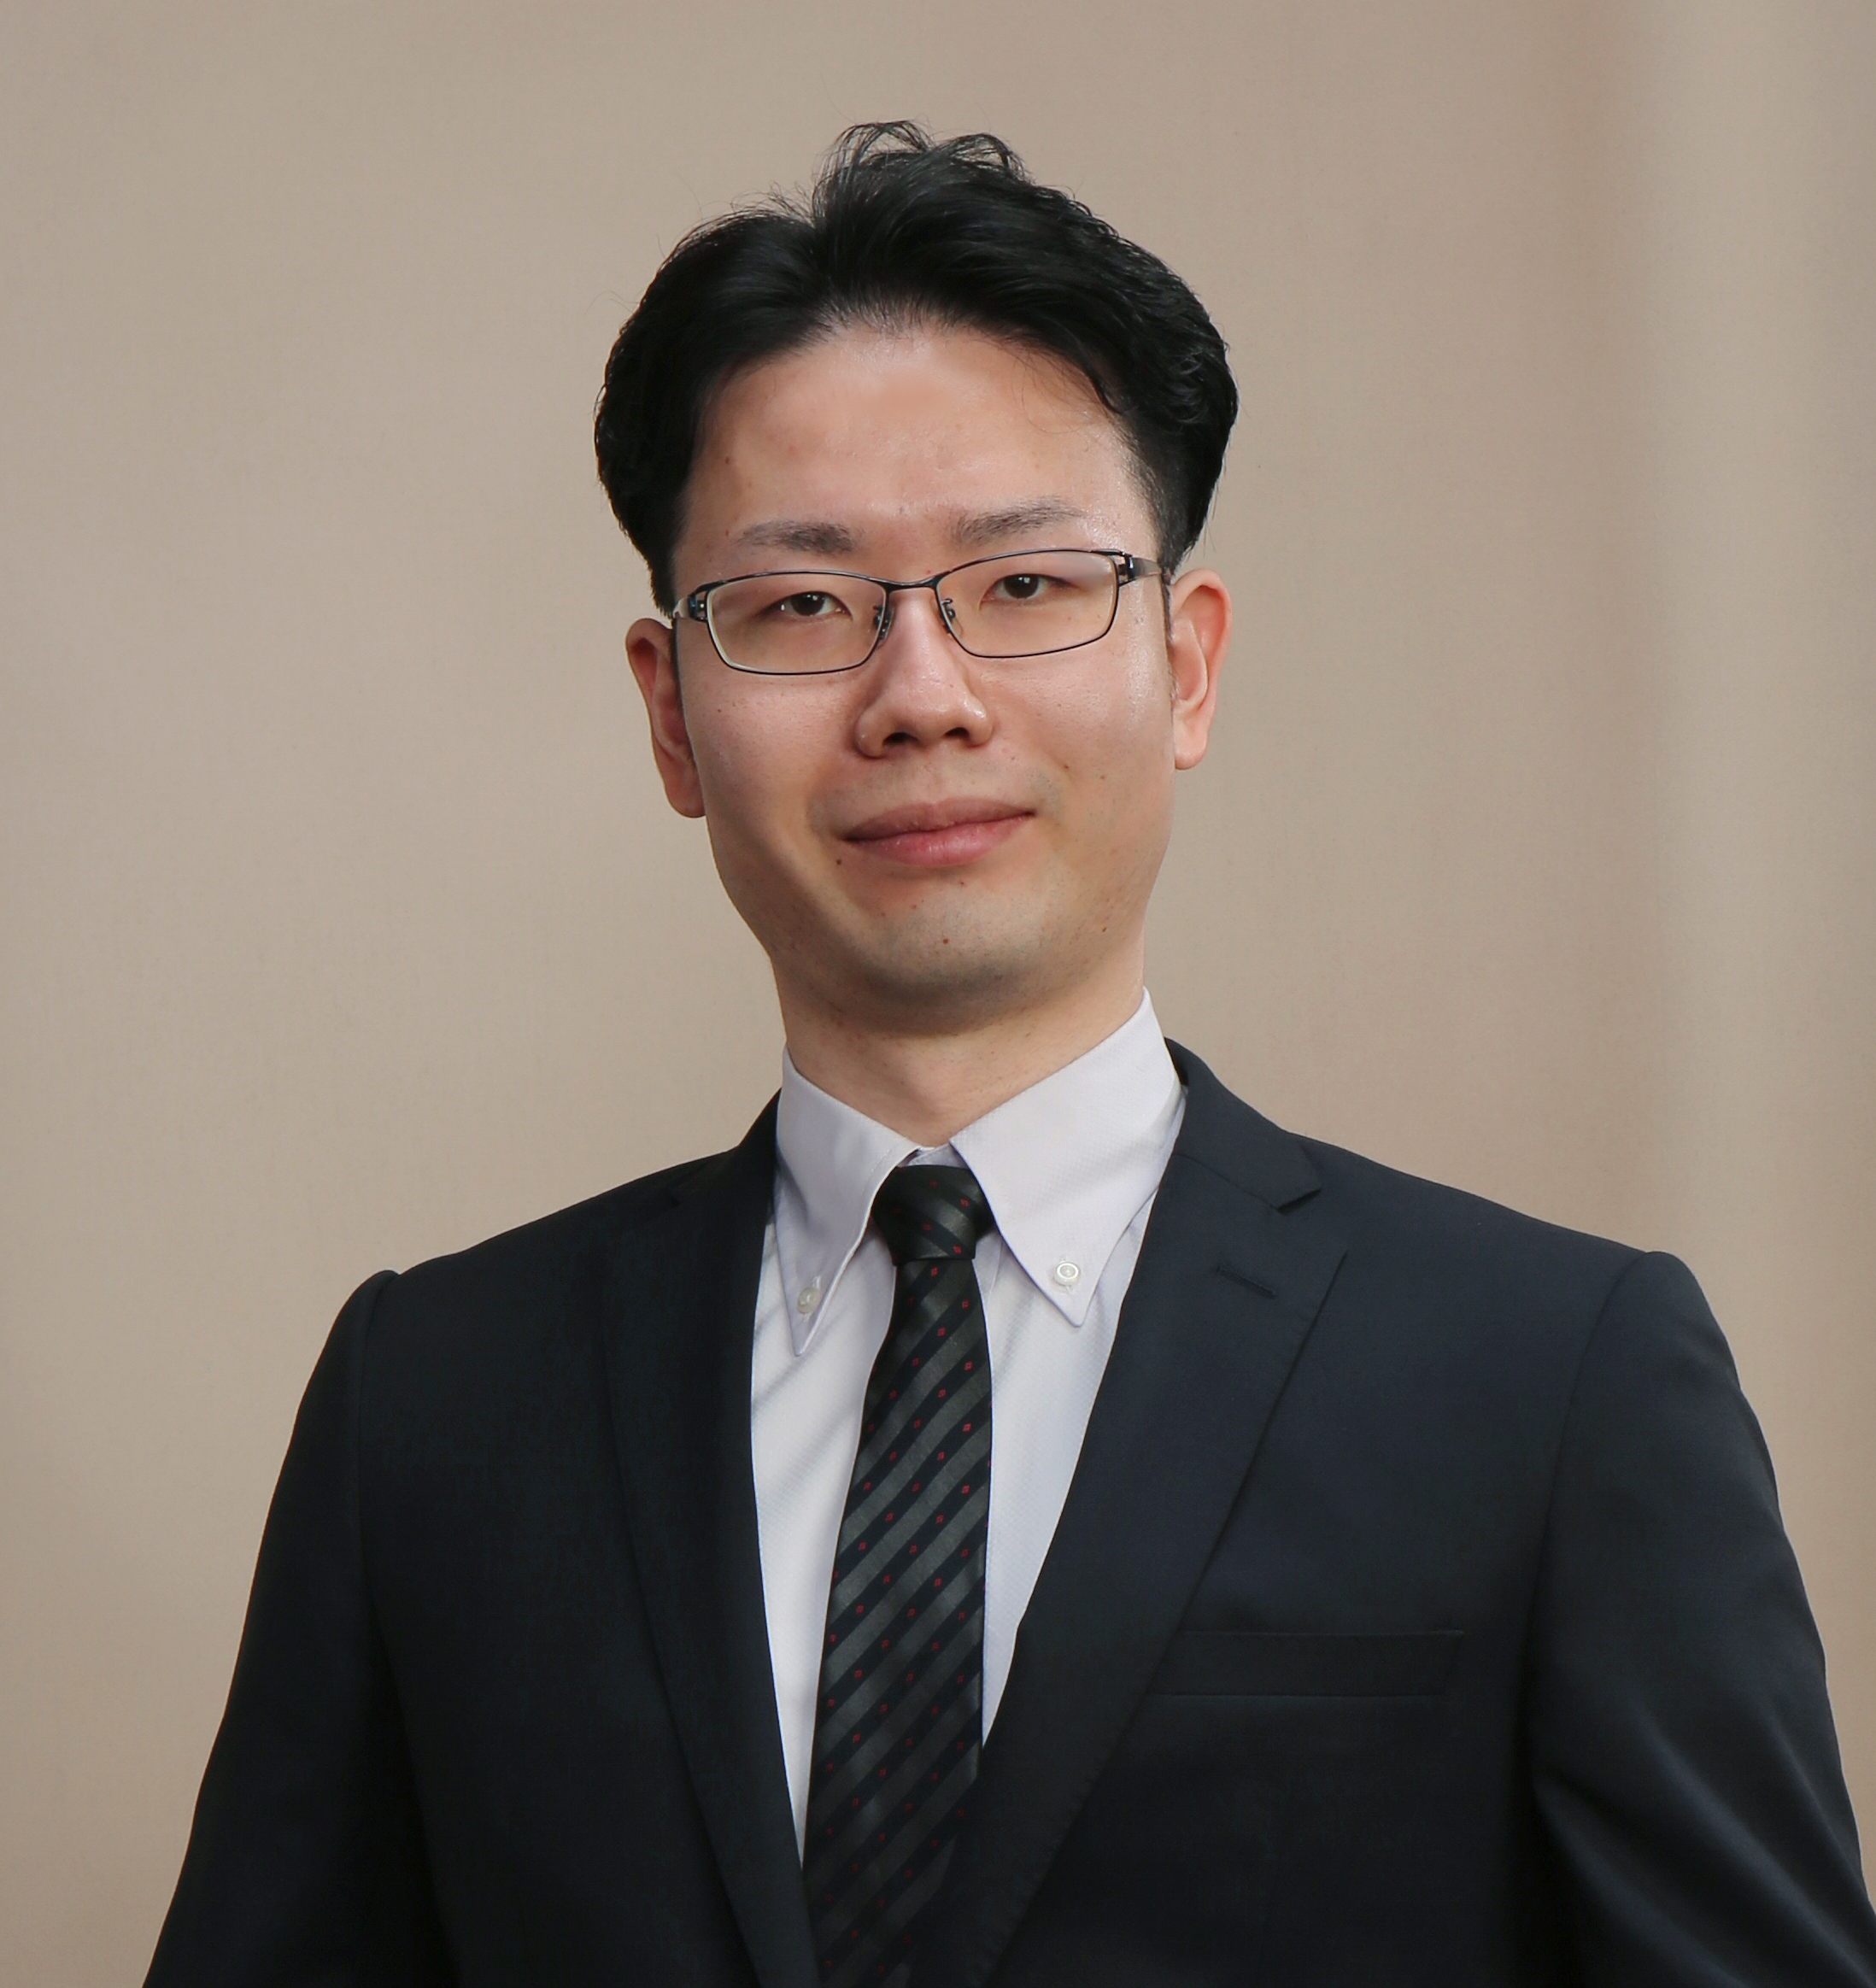
\includegraphics[width=3cm]{photo.jpg}
\end{minipage}
\vspace{4pt}

% ======================================================================
\section{Research Interests}
Supporting software developers by providing tools and methods for software quality assurance activities based on mining software repositories, machine learning, and statistical analysis techniques. Topics include software defect prediction, SZZ and issue-link algorithms, automated program repair, LLMs for software engineering, and empirical studies of open-source software development.

% ======================================================================
\section{Academic Appointments}
\entry{Apr.\ 2021 -- present}{\textbf{Assistant Professor}, Principles of Software engineering and programming Languages Lab.\ (POSL), Graduate School and Faculty of Information Science and Electrical Engineering, Kyushu University, Japan}
\entry{2025 -- present}{\textbf{Project Researcher}, National Institute of Informatics (NII), Japan (concurrent position)}
\entry{Apr.\ 2019 -- Mar.\ 2021}{\textbf{JSPS Research Fellow (DC1)}, Japan Society for the Promotion of Science}
\entry{Mar.\ 2018 -- Mar.\ 2019}{\textbf{Visiting Researcher}, Software Analysis \& Intelligence Lab (SAIL), Queen's University, Kingston, Canada (Host: Prof.\ Ahmed E.\ Hassan). Supported as a Young Ambassador of the ``TOBITATE! Young Ambassador Program''}

% ======================================================================
\section{Education}
\entry{2021}{\textbf{Ph.D.\ (Dr.\ Eng.)}, Graduate School of Science and Technology, Kyoto Institute of Technology, Japan\newline
  Supervisor: Prof.\ Osamu Mizuno\newline
  Thesis: \textit{An Empirical Study of Feature Engineering on Software Defect Prediction}}
\entry{2019}{\textbf{M.Sc.}, Graduate School of Science and Technology, Kyoto Institute of Technology, Japan\newline
  Thesis: \textit{The Impact of Feature Reduction Techniques on Defect Prediction Models}}
\entry{2017}{\textbf{B.Sc.}, Kyoto Institute of Technology, Japan\newline
  Thesis: \textit{Feature Extraction of Software Metrics Using RBMs} \inJP}

% ======================================================================
\section{Research Grants}
\entry{Apr.\ 2025 -- Mar.\ 2029}{\textbf{Principal Investigator}, JSPS KAKENHI Grant-in-Aid for Scientific Research (B) (25K03100), ``Rationale Mining for Supporting Code Comprehension of Existing Software,'' direct costs: JPY 14,500,000.}
\entry{Dec.\ 2024 -- Mar.\ 2028}{\textbf{Lead Co-Investigator}, JST ASPIRE (Adopting Sustainable Partnerships for Innovative Research Ecosystem) (JPMJAP2415), ``International Brain Circulation toward Context-Aware AI for Software Development,'' direct costs: JPY 69,230,000.}
\entry{Apr.\ 2024 -- Mar.\ 2028}{\textbf{Co-Investigator}, JSPS KAKENHI Grant-in-Aid for Scientific Research (B) (24K02921), ``Fault Localization from Incomplete System Logs: Toward Automated System Recovery,'' direct costs: JPY 14,300,000.}
\entry{Apr.\ 2022 -- Mar.\ 2025}{\textbf{Principal Investigator}, JSPS KAKENHI Grant-in-Aid for Early-Career Scientists (22K17874), ``Just-in-Time Automated Program Repair for Discovering and Fixing Latent Bugs,'' direct costs: JPY 3,500,000.}
\entry{Apr.\ 2019 -- Mar.\ 2021}{\textbf{Principal Investigator}, JSPS Grant-in-Aid for JSPS Fellows (19J23477), ``Software Defect Detection Using Deep Learning on Individual Developer Activities,'' direct costs: JPY 1,900,000.}

% ======================================================================
\section{Awards and Honors}
\subsection{Awards Received}
\entry{Mar.\ 2026}{The 30th (FY2025) JSEE Award for Engineering Education (Achievement Category), Japanese Society for Engineering Education, for ``Discovering and Developing Next-Generation Engineers in Fukuoka Prefecture'' (team led by Prof.\ Yutaka Arakawa, Kyushu University; participated as Project Manager)}
\entry{Feb.\ 2026}{Best Paper Award and Best Presentation Award, rePiT 2026, for ``PointerPuzzle: A Learning Support Game for C Pointers and Its Preliminary Evaluation''}
\entry{Sep.\ 2025}{IPSJ SIGSE Distinguished Research Award, for ``An Empirical Study of Token-based Micro Commits'' (EMSE, 2024)}
\entry{Sep.\ 2025}{IPSJ SIGSE Distinguished Research Award, for ``Repairs and Breaks Prediction for Deep Neural Networks'' (TOSEM, 2025)}
\entry{Sep.\ 2025}{Research Encouragement Award, SES 2025, for ``Differences in Software Engineering Education between Japan and Other Countries Seen from Syllabi: A Comparison with World Top Universities''}
\entry{Apr.\ 2024}{Distinguished Reviewer Award, ICPC 2024 Research Track}
\entry{Sep.\ 2020}{IPSJ SIGSE Distinguished Research Award, for ``Code Cloning in Smart Contracts: A Case Study on Verified Contracts from the Ethereum Blockchain Platform'' (EMSE, 2020)}
\entry{Aug.\ 2019}{IPSJ SIGSE Distinguished Research Award, for ``The Impact of Feature Reduction Techniques on Defect Prediction Models'' (EMSE, 2019)}
\entry{Aug.\ 2019}{IPSJ SIGSE Distinguished Research Award, for ``The Impact of Context Metrics on Just-In-Time Defect Prediction'' (EMSE, 2020)}
\entry{Mar.\ 2019}{Research Achievement Award, Graduate School of Science and Technology, Kyoto Institute of Technology}
\entry{Mar.\ 2019}{IPSJ Yamashita SIG Research Award, for ``Prediction and Evaluation of Fault-Inducing Commits Using Deep Learning'' (SES 2017)}
\entry{Apr.\ 2018}{IPSJ Specially Selected Paper, for ``Fault-Inducing Prediction from Source Code Commits Using Deep Learning'' (IPSJ Journal, 59(4), 2018)}
\entry{Mar.\ 2018}{Zengo Award, NPO ASTER, for ``Prediction and Evaluation of Fault-Inducing Commits Using Deep Learning'' (SES 2017)}
\entry{Sep.\ 2017}{Best Paper Award, Software Engineering Symposium 2017 (SES 2017)}

\subsection{Awards Received by Supervised Students}
\entry{Mar.\ 2026}{IPSJ Computer Science Research Award for Young Scientists (FY2026), awarded to Sota Nakashima, for ``Automated Construction of SATD Taxonomies Using Large Language Models'' (IPSJ SIGSE 220th, 2025)}
\entry{Mar.\ 2026}{IEICE SIGSS Research Encouragement Award (FY2025), awarded to Inase Kondo, for ``An Initial Study of an SZZ Method with Search Scope Extended by Function Dependencies''}
\entry{Mar.\ 2025}{IEICE SIGSS Research Encouragement Award (FY2024), awarded to Kazuki Kusama, for ``An Empirical Study of Automated Program Repair Using Small Language Models''}
\entry{Nov.\ 2024}{Poster/Demo Award, FOSE 2024, awarded to Yuta Ishimoto, for ``Repairs and Breaks Prediction for Deep Neural Networks''}
\entry{Nov.\ 2023}{IEEE Computer Society Japan Chapter FOSE Young Researcher Award, awarded to Kaito Utsunomiya (FOSE 2023)}
\entry{Mar.\ 2023}{IPSJ SIGSE Student Research Award (213th meeting), awarded to Jianhong Wang}
\entry{Nov.\ 2022}{IEEE Computer Society Japan Chapter FOSE Young Researcher Award, awarded to Yuto Nakamura (FOSE 2022)}
\entry{Mar.\ 2022}{IPSJ SIGSE Student Research Award (210th meeting), awarded to Yuto Nakamura}
\entry{Nov.\ 2021}{IEEE Computer Society Japan Chapter FOSE Young Researcher Award, awarded to Yuga Matsuda (FOSE 2021)}
\entry{Sep.\ 2021}{Research Encouragement Award, SES 2021, awarded to Tsukasa Nakamura}
\entry{Sep.\ 2021}{Student Encouragement Award, SES 2021, awarded to Kentaro Okino}
\entry{Aug.\ 2019}{IEEE Computer Society Japan Chapter SES Young Researcher Award, awarded to Sayaka Kitamura (SES 2019)}

% ======================================================================
\section{Publications}
\subsection{Books}
\begin{publist}[label={[B\arabic*]}]
  \item Hironori Washizaki (ed.), \me, et al.\ (12 authors), \textit{Software Development with Generative AI: A Practical Framework for Using LLMs to Transform Everything from Design to Testing and Management}, supervised by IPSJ, Ohmsha, Nov.\ 2025. ISBN: 978-4-274-23415-6. \inJP
  \item Contributor, \textit{OSS Myths and Facts}, 2024. \url{https://arxiv.org/abs/2404.09223}
\end{publist}

\subsection{Refereed Journal Articles (International)}
\begin{publist}[label={[J\arabic*]}]
  \item Haruka Tokumasu, \me, Alexander Serebrenik, Dong Wang, Kei Koyanagi, Kotaro Noguchi, Naoyasu Ubayashi, Yasutaka Kamei, ``A Study on the Impact of Natural Language Differences in Prompts on Automatic Code Generation Using LLMs,'' \textit{Empirical Software Engineering}, 2026 (accepted, to appear).
  \item Inase Kondo, \me, Daniel M.\ German, Yasutaka Kamei, Yoshiki Higo, ``MV-SZZ: A Majority Voting-Based SZZ Method,'' \textit{IEEE Transactions on Software Engineering}, vol.\ 52, no.\ 6, pp.\ 1911--1927, 2026. doi:\nolinkurl{10.1109/TSE.2026.3688089}
  \item Jianchen Zhao, Kundi Yao, \me, Hetong Dai, Weiyi Shang, Yasutaka Kamei, ``Not-So-Pretty: Studying and Segmenting Multiline Console Logs,'' \textit{ACM Transactions on Software Engineering and Methodology}, 2026. doi:\nolinkurl{10.1145/3803019}
  \item Olivier Nourry, \me, Shinobu Saito, Yukako Iimura, Naoyasu Ubayashi, Yasutaka Kamei, ``Abandonment and Resilience: Understanding Core Developer Turnover in Open Source Software,'' \textit{IEICE Transactions on Information and Systems}, vol.\ E108-D, no.\ 11, pp.\ 1412--1415, 2025. doi:\nolinkurl{10.1587/transinf.2025EDL8005}
  \item Yuta Ishimoto, \me, Lei Ma, Naoyasu Ubayashi, Yasutaka Kamei, ``Repairs and Breaks Prediction for Deep Neural Networks,'' \textit{ACM Transactions on Software Engineering and Methodology}, vol.\ 34, no.\ 4, article 94, pp.\ 1--42, 2025. doi:\nolinkurl{10.1145/3702983}
  \item \me, Daniel M.\ German, Yasutaka Kamei, Naoyasu Ubayashi, Osamu Mizuno, ``An Empirical Study of Token-based Micro Commits,'' \textit{Empirical Software Engineering}, vol.\ 29, no.\ 148, 2024.
  \item Hiroki Kuramoto, Dong Wang, \me, Yutaro Kashiwa, Yasutaka Kamei, Naoyasu Ubayashi, ``Understanding the Characteristics and the Role of Visual Issue Reports,'' \textit{Empirical Software Engineering}, vol.\ 29, no.\ 89, 2024.
  \item Dong Wang, \me, Yasutaka Kamei, Raula Gaikovina Kula, Naoyasu Ubayashi, ``When Conversations Turn Into Work: A Taxonomy of Converted Discussions and Issues in GitHub,'' \textit{Empirical Software Engineering}, vol.\ 28, no.\ 138, 2023.
  \item Yuta Ishimoto, \me, Naoyasu Ubayashi, Yasutaka Kamei, ``PAFL: Probabilistic Automaton-based Fault Localization for Recurrent Neural Networks,'' \textit{Information and Software Technology}, vol.\ 155, 2023.
  \item Khine Yin Mon, \me, Eunjong Choi, Osamu Mizuno, ``Commit-based Class-level Defect Prediction for Python Projects,'' \textit{IEICE Transactions on Information and Systems}, vol.\ E106-D, no.\ 2, pp.\ 157--165, 2023.
  \item \me, Yutaro Kashiwa, Yasutaka Kamei, Osamu Mizuno, ``An Empirical Study of Issue-Link Algorithms: Which Issue-Link Algorithms Should We Use?,'' \textit{Empirical Software Engineering}, vol.\ 27, no.\ 136, 2022.
  \item Yutaro Kashiwa, Ryoma Nishikawa, Yasutaka Kamei, \me, Emad Shihab, Ryosuke Sato, Naoyasu Ubayashi, ``An Empirical Study on Self-Admitted Technical Debt in Modern Code Review,'' \textit{Information and Software Technology}, vol.\ 146, 2022.
  \item \me, Gustavo A.\ Oliva, Zhen Ming (Jack) Jiang, Ahmed E.\ Hassan, Osamu Mizuno, ``Code Cloning in Smart Contracts: A Case Study on Verified Contracts from the Ethereum Blockchain Platform,'' \textit{Empirical Software Engineering}, vol.\ 25, no.\ 6, pp.\ 4617--4675, 2020. doi:\nolinkurl{10.1007/s10664-020-09852-5}
  \item \me, Daniel M.\ German, Osamu Mizuno, Eun-Hye Choi, ``The Impact of Context Metrics on Just-In-Time Defect Prediction,'' \textit{Empirical Software Engineering}, vol.\ 25, no.\ 1, pp.\ 890--939, 2020. doi:\nolinkurl{10.1007/s10664-019-09736-3}
  \item \me, Cor-Paul Bezemer, Yasutaka Kamei, Ahmed E.\ Hassan, Osamu Mizuno, ``The Impact of Feature Reduction Techniques on Defect Prediction Models,'' \textit{Empirical Software Engineering}, vol.\ 24, no.\ 4, pp.\ 1925--1963, 2019. doi:\nolinkurl{10.1007/s10664-018-9679-5}
  \item \me, Osamu Mizuno, Eun-Hye Choi, ``Causal-Effect Analysis Using Bayesian LiNGAM Comparing with Correlation Analysis in Function Point Metrics and Effort,'' \textit{International Journal of Mathematical, Engineering and Management Sciences (IJMEMS)}, vol.\ 3, no.\ 2, pp.\ 90--112, 2018.
\end{publist}

\subsection{Refereed International Conference and Workshop Papers}
\begin{publist}[label={[C\arabic*]}]
  \item Napasorn Lapprakobkit, \me, Tao Xiao, Morakot Choetkiertikul, Chaiyong Ragkhitwetsagul, Pattaraporn Sangaroonsilp, Thanwadee Sunetnanta, Yasutaka Kamei, ``Quantifying the Resolved Tasks and Cost That Test Feedback Adds to LLM-Based Program Repair,'' In \textit{Proc.\ of the 13th International Workshop on Quantitative Approaches to Software Quality (QuASoQ 2026)}, 2026 (accepted, to appear).
  \item Napasorn Lapprakobkit, Haruka Tokumasu, Tao Xiao, \me, Morakot Choetkiertikul, Chaiyong Ragkhitwetsagul, Yasutaka Kamei, ``Early Adoption, Use, and Maintenance of the Agent Package Manager in Open-Source Software,'' In \textit{Proc.\ of the 33rd Asia-Pacific Software Engineering Conference (APSEC 2026), ERA Track}, 2026 (accepted, to appear). Acceptance rate: 40.8\% (20/49).
  \item Taiki Wakamatsu, Yuta Ishimoto, \me, Yasutaka Kamei, ``PreMaQ: Predicting Maintainability-Related Quality of LLM-Generated Code Before Generation,'' In \textit{Proc.\ of the 33rd Asia-Pacific Software Engineering Conference (APSEC 2026), Technical Track}, 2026 (accepted, to appear).
  \item Sota Nakashima, Yuta Ishimoto, \me, Tao Xiao, Yasutaka Kamei, ``How Well Do LLMs Generate Taxonomies in the SE Domain? A Multi-Perspective Evaluation Framework,'' In \textit{Proc.\ of the 41st IEEE/ACM International Conference on Automated Software Engineering (ASE 2026)}, pp.\ 3239--3251, 2026.
  \item Ayane Shirakawa, Tatsuya Shirai, Yutaro Kashiwa, \me, Yasutaka Kamei, Hajimu Iida, ``Test Alert Snooze: An Empirical Study of Consecutive Test Failures on CI,'' In \textit{Proc.\ of the 20th ACM/IEEE International Symposium on Empirical Software Engineering and Measurement (ESEM 2026)}, 2026 (accepted, to appear).
  \item Yuta Ishimoto, Paolo Arcaini, Fuyuki Ishikawa, \me, Naoyasu Ubayashi, Yasutaka Kamei, ``RepTran: Search-Based Repair of Transformer Models,'' In \textit{Proc.\ of the 37th IEEE International Symposium on Software Reliability Engineering (ISSRE 2026)}, 2026 (accepted, to appear).
  \item Yuki Toi, Tao Xiao, Kazushi Tomoto, \me, Yasutaka Kamei, ``Exploring the Potential of Program Flowcharts on Code Generation Using Multimodal LLMs,'' In \textit{Proc.\ of the 26th IEEE International Conference on Software Quality, Reliability, and Security (QRS 2026)}, 2026 (accepted, to appear).
  \item Kazuki Kusama, Honglin Shu, \me, Tao Xiao, Yasutaka Kamei, ``ThinkLog: Leveraging Reasoning for Log Statement Generation,'' In \textit{Proc.\ of the 26th IEEE International Conference on Software Quality, Reliability, and Security (QRS 2026), Short Paper}, 2026 (accepted, to appear).
  \item Sota Nakashima, \me, Mahmoud Alfadel, Aly Ahmad, Toshihiro Nakae, Hidenori Matsuzaki, Yasutaka Kamei, ``Toward Linking Declined Proposals and Source Code: An Exploratory Study on the Go Repository,'' In \textit{Proc.\ of the 23rd International Conference on Mining Software Repositories (MSR 2026)}, 2026 (accepted, to appear).
  \item Chihiro Yoshida, Yuta Ishimoto, Olivier Nourry, \me, Makoto Matsushita, Yasutaka Kamei, Yoshiki Higo, ``Leveraging Mutation Analysis for LLM-based Repair of Quantum Programs,'' In \textit{Proc.\ of the 33rd IEEE International Conference on Software Analysis, Evolution and Reengineering (SANER 2026)}, pp.\ 92--97, 2026. doi:\nolinkurl{10.1109/SANER67736.2026.00019}
  \item Ayana Uematsu, Hironori Washizaki, Naoyasu Ubayashi, \me, Juichi Takahashi, Yohei Takagi, ``BUPLinker: Bridging Users and Developers in Mobile Application Evolution,'' In \textit{Proc.\ of the 33rd IEEE International Conference on Software Analysis, Evolution and Reengineering (SANER 2026)}, pp.\ 485--490, 2026. doi:\nolinkurl{10.1109/SANER67736.2026.00059}
  \item Ryo Masuda, Takahiro Kinoshita, Hideyuki Kanuka, Sien Reeve O.\ Peralta, Hironori Washizaki, \me, ``Revealing Reversed Causal Effects in Bug-Fix Delays: A LiNGAM-Based Comparison between OSS and Enterprise Systems,'' In \textit{Proc.\ of the 33rd IEEE International Conference on Software Analysis, Evolution and Reengineering (SANER 2026)}, pp.\ 1034--1039, 2026. doi:\nolinkurl{10.1109/SANER67736.2026.00121}
  \item Panya Trakoolgerntong, Tao Xiao, \me, Chaiyong Ragkhitwetsagul, Morakot Choetkiertikul, Pattaraporn Sangaroonsilp, Yasutaka Kamei, ``AILINKPREVIEWER: Enhancing Code Reviews with LLM-Powered Link Previews,'' In \textit{Proc.\ of the 32nd Asia-Pacific Software Engineering Conference (APSEC 2025)}, pp.\ 1021--1024, 2025. doi:\nolinkurl{10.1109/APSEC66846.2025.00121}
  \item Sota Nakashima, Yuta Ishimoto, \me, Tao Xiao, Yasutaka Kamei, ``How Far Have LLMs Come Toward Automated SATD Taxonomy Construction?,'' In \textit{Proc.\ of the 32nd Asia-Pacific Software Engineering Conference (APSEC 2025)}, pp.\ 832--836, 2025. doi:\nolinkurl{10.1109/APSEC66846.2025.00087}
  \item Chunrun Tao, Honglin Shu, \me, Yasutaka Kamei, ``A Preliminary Study on Large Language Models Self-Negotiation in Software Engineering,'' In \textit{Proc.\ of the 41st International Conference on Software Maintenance and Evolution (ICSME 2025)}, pp.\ 833--838, 2025. doi:\nolinkurl{10.1109/ICSME64153.2025.00088}
  \item Kazuki Kusama, Honglin Shu, \me, Yasutaka Kamei, ``How Small is Enough? Empirical Evidence of Quantized Small Language Models for Automated Program Repair,'' In \textit{Proc.\ of the 19th ACM/IEEE International Symposium on Empirical Software Engineering and Measurement (ESEM 2025)}, pp.\ 393--399, 2025. doi:\nolinkurl{10.1109/ESEM64174.2025.00047}
  \item Yuta Ishimoto, \me, Naoyasu Ubayashi, Yasutaka Kamei, Ryota Katsube, Naoto Sato, Hideto Ogawa, ``Evaluating Mutation-based Fault Localization for Quantum Programs,'' In \textit{Proc.\ of the 29th International Conference on Evaluation and Assessment in Software Engineering (EASE 2025)}, pp.\ 666--671, 2025. doi:\nolinkurl{10.1145/3756681.3757022}
  \item Yuta Ishimoto, Yuto Nakamura, Ryota Katsube, Naoto Sato, Hideto Ogawa, \me, Yasutaka Kamei, Naoyasu Ubayashi, ``An Empirical Study on Self-Admitted Technical Debt in Quantum Software,'' In \textit{Proc.\ of the 31st Asia-Pacific Software Engineering Conference (APSEC 2024)}, pp.\ 41--50, 2024. doi:\nolinkurl{10.1109/APSEC65559.2024.00015}
  \item Olivier Nourry, \me, Mahmoud Alfadel, Shane McIntosh, Yasutaka Kamei, ``Exploring the Adoption of Fuzz Testing in Open-Source Software: A Case Study of the Go Community,'' In \textit{Proc.\ of the 40th International Conference on Software Maintenance and Evolution (ICSME 2024)}, pp.\ 300--311, 2024.
  \item Kei Koyanagi, Dong Wang, Kotaro Noguchi, \me, Alexander Serebrenik, Yasutaka Kamei, Naoyasu Ubayashi, ``Exploring the Effect of Multiple Natural Languages on Code Suggestion Using GitHub Copilot,'' In \textit{Proc.\ of the 21st International Conference on Mining Software Repositories (MSR 2024)}, pp.\ 481--486, 2024.
  \item Issei Morita, Yutaro Kashiwa, \me, Jeongju Sohn, Shane McIntosh, Yasutaka Kamei, Naoyasu Ubayashi, ``TraceJIT: Evaluating the Impact of Behavioral Code Change on Just-In-Time Defect Prediction,'' In \textit{Proc.\ of the IEEE International Conference on Software Analysis, Evolution and Reengineering (SANER 2024)}, pp.\ 580--591, 2024.
  \item Hiroya Watanabe, \me, Eunjong Choi, Osamu Mizuno, ``Benefits and Pitfalls of Token-Level SZZ: An Empirical Study on OSS Projects,'' In \textit{Proc.\ of the IEEE International Conference on Software Analysis, Evolution and Reengineering (SANER 2024)}, pp.\ 776--786, 2024.
  \item \me, Shinobu Saito, Yukako Iimura, Eunjong Choi, Osamu Mizuno, Yasutaka Kamei, Naoyasu Ubayashi, ``Towards Better Online Communication for Future Software Development in Industry,'' In \textit{Proc.\ of the 17th IEEE International Workshop on Quality Oriented Reuse of Software (QUORS 2023)}, pp.\ 1619--1624, 2023.
  \item Yuta Ishimoto, Ken Matsui, \me, Naoyasu Ubayashi, Yasutaka Kamei, ``An Initial Analysis of Repair and Side-effect Prediction for Neural Networks,'' In \textit{Proc.\ of the 2nd International Conference on AI Engineering -- Software Engineering for AI (CAIN 2023)}, pp.\ 80--85, 2023.
  \item Hiroki Yamamoto, Dong Wang, Gopi Krishnan Rajbahadur, \me, Yasutaka Kamei, Naoyasu Ubayashi, ``Towards Privacy Preserving Cross Project Defect Prediction with Federated Learning,'' In \textit{Proc.\ of the IEEE International Conference on Software Analysis, Evolution and Reengineering (SANER 2023)}, pp.\ 485--496, 2023.
  \item Jianhong Wang, Yuta Ishimoto, \me, Yasutaka Kamei, Naoyasu Ubayashi, ``Uncertainty-Aware Metamorphic Testing for Robust Object Detection Models,'' In \textit{Proc.\ of the 23rd IEEE International Conference on Software Quality, Reliability and Security Companion (QRS-C 2023)}, 2023. doi:\nolinkurl{10.1109/QRS-C60940.2023.00058}
  \item Kyosuke Yamate, \me, Yutaro Kashiwa, Yasutaka Kamei, Naoyasu Ubayashi, ``Hey APR! Integrate Our Fault Localization Skill: Toward Better Automated Program Repair,'' In \textit{Proc.\ of the IEEE Computers, Software, and Applications Conference (COMPSAC 2022)}, pp.\ 563--568, 2022.
  \item Tsukasa Nakamura, \me, Yasutaka Kamei, Naoyasu Ubayashi, ``Evaluating Automated Program Repair Techniques using Introductory Programming Course Datasets,'' In \textit{Proc.\ of the IEEE Computers, Software, and Applications Conference (COMPSAC 2022)}, pp.\ 569--574, 2022.
  \item Hiroki Kuramoto, \me, Yutaro Kashiwa, Yuta Ishimoto, Kaze Shindo, Yasutaka Kamei, Naoyasu Ubayashi, ``Do Visual Issue Reports Help Developers Fix Bugs? A Preliminary Study of Using Videos and Images to Report Issues on GitHub,'' In \textit{Proc.\ of the 30th IEEE/ACM International Conference on Program Comprehension (ICPC 2022), ERA Track}, pp.\ 511--515, 2022.
  \item \me, Shinobu Saito, Yukako Iimura, Eunjong Choi, Osamu Mizuno, Yasutaka Kamei, Naoyasu Ubayashi, ``Challenges and Future Research Direction for Microtask Programming in Industry,'' In \textit{Proc.\ of the 19th International Conference on Mining Software Repositories (MSR 2022), Industry Track}, pp.\ 103--104, 2022.
  \item Lei Shi, \me, Naoyasu Ubayashi, Yasutaka Kamei, ``Towards Better Coverage of Dataset with Software Product Line Engineering,'' In \textit{Proc.\ of the 21st IEEE International Conference on Software Quality, Reliability, and Security Companion (QRS-C 2021)}, pp.\ 1173--1174, 2021.
  \item Shoma Kokuryo, \me, Osamu Mizuno, ``An Empirical Study of Utilization of Imperative Modules in Ansible,'' In \textit{Proc.\ of the 20th IEEE International Conference on Software Quality, Reliability, and Security (QRS 2020)}, pp.\ 442--449, 2020.
  \item Kai Yamamoto, \me, Kinari Nishiura, Osamu Mizuno, ``Which Metrics Should Researchers Use to Collect Repositories: An Empirical Study,'' In \textit{Proc.\ of the 20th IEEE International Conference on Software Quality, Reliability, and Security (QRS 2020)}, pp.\ 458--466, 2020.
  \item Juntong Hong, Osamu Mizuno, \me, ``An Empirical Study of Source Code Detection Using Image Classification,'' In \textit{Proc.\ of the 10th International Workshop on Empirical Software Engineering in Practice (IWESEP 2019)}, pp.\ 1--7, 2019.
  \item \me, Osamu Mizuno, ``Analysis on Causal-Effect Relationship in Effort Metrics Using Bayesian LiNGAM,'' In \textit{Proc.\ of the 27th International Symposium on Software Reliability Engineering (ISSRE 2016), Workshops}, pp.\ 47--48, Ottawa, Canada, Oct.\ 2016.
  \item \me, Ryosuke Kubota, ``A Modified Genetic Algorithm for Nurse Scheduling Problem with Considering Individual Preference,'' In \textit{Proc.\ of the International Symposium on Technology for Sustainability (ISTS 2014)}, 4 pages, Taipei, Taiwan, Nov.\ 2014.
\end{publist}

\subsection{Theses}
\begin{publist}[label={[T\arabic*]}]
  \item \me, ``An Empirical Study of Feature Engineering on Software Defect Prediction,'' Ph.D.\ thesis, Graduate School of Science and Technology, Kyoto Institute of Technology, 2021.
  \item \me, ``The Impact of Feature Reduction Techniques on Defect Prediction Models,'' Master's thesis, Graduate School of Science and Technology, Kyoto Institute of Technology, 2019.
  \item \me, ``Feature Extraction of Software Metrics Using RBMs,'' Bachelor's thesis, Kyoto Institute of Technology, Feb.\ 2017. \inJP
\end{publist}

% ======================================================================
\section{Presentations and Invited Talks}
\subsection{Invited Talks}
\entry{Sep.\ 2026}{``An Empirical Study of Token-based Micro Commits,'' Top Conference Session, the 25th Forum on Information Technology (FIT 2026). \inJP}
\entry{Sep.\ 2024}{``Benefits and Pitfalls of Token-Level SZZ: An Empirical Study on OSS Projects,'' Invited Paper Session, Software Engineering Symposium 2024 (SES 2024).}
\entry{Sep.\ 2023}{``Toward Mining Software Repositories Research Appreciated by Developers,'' Special Lecture by Young Researchers (40th Anniversary Session), the 40th Annual Conference of the Japan Society for Software Science and Technology (JSSST). \inJP}
\entry{Sep.\ 2023}{``An Empirical Study of Issue-Link Algorithms: Which Issue-Link Algorithms Should We Use?,'' Special Lecture on Top Conference and Journal Papers, the 40th Annual Conference of JSSST.}
\entry{Sep.\ 2023}{``An Empirical Study of Issue-Link Algorithms,'' Top Conference Session, the 22nd Forum on Information Technology (FIT 2023). \inJP}
\entry{Aug.\ 2023}{``Towards Privacy Preserving Cross Project Defect Prediction with Federated Learning,'' Invited Paper Session, SES 2023.}
\entry{Aug.\ 2023}{``An Empirical Study of Issue-Link Algorithms: Which Issue-Link Algorithms Should We Use?,'' Invited Paper Session, SES 2023.}
\entry{Nov.\ 2021}{``Feature Engineering in Software Defect Prediction and Future Perspectives,'' Invited talk for the IPSJ Recommended Doctoral Dissertation, the 209th IPSJ SIGSE Meeting. \inJP}
\entry{Sep.\ 2021}{AI TechPlay Seminar (AI edition), Dell Technologies $\times$ NAIST $\times$ dTosh.}
\entry{Aug.\ 2019}{``The Impact of Feature Reduction Techniques on Defect Prediction Models'' and ``The Impact of Context Metrics on Just-In-Time Defect Prediction,'' IPSJ SIGSE Distinguished Research Award Paper Session, SES 2019.}

\subsection{International Conference Presentations}
\entry{Jun.\ 2025}{``An Empirical Study of Token-based Micro Commits,'' Journal First Track, ACM International Conference on the Foundations of Software Engineering (FSE 2025).}
\entry{Mar.\ 2024}{``Benefits and Pitfalls of Token-Level SZZ: An Empirical Study on OSS Projects,'' IEEE International Conference on Software Analysis, Evolution and Reengineering (SANER 2024).}
\entry{Jun.\ 2023}{``Towards Better Online Communication for Future Software Development in Industry,'' the 17th IEEE International Workshop on Quality Oriented Reuse of Software (QUORS 2023).}
\entry{May 2023}{``An Empirical Study of Issue-Link Algorithms: Which Issue-Link Algorithms Should We Use?,'' Journal First Track, International Conference on Software Engineering (ICSE 2023).}
\entry{May 2022}{``Challenges and Future Research Direction for Microtask Programming in Industry,'' Industry Track, International Conference on Mining Software Repositories (MSR 2022).}
\entry{Jul.\ 2020}{``The Impact of Feature Reduction Techniques on Defect Prediction Models,'' Journal First Track, International Conference on Software Engineering (ICSE 2020) (virtual).}
\entry{Sep.\ 2019}{``The Impact of Context Metrics on Just-In-Time Defect Prediction,'' Journal First Track, International Conference on Software Maintenance and Evolution (ICSME 2019).}
\entry{Oct.\ 2016}{``Analysis on Causal-Effect Relationship in Effort Metrics Using Bayesian LiNGAM,'' Fast Abstract Track, International Symposium on Software Reliability Engineering (ISSRE 2016).}
\entry{Nov.\ 2014}{``A Modified Genetic Algorithm for Nurse Scheduling Problem with Considering Individual Preference,'' International Symposium on Technology for Sustainability (ISTS 2014).}

% ======================================================================
\section{Professional Service}
\subsection{Organizing Committees of International Conferences}
\entry{2027}{Registered Reports Track Co-Chair, International Conference on Mining Software Repositories (MSR 2027)}
\entry{2025}{General Chair, AI-Driven Software Engineering Summit for Fostering Next-Generation Researchers}
\entry{2024}{Program Co-Chair, the First International Symposium on the Future of Software Engineering}
\entry{2023, 2024}{General Chair, Exploring Employee Experience in Open Source Software (EEE-OSS 2023, EEE-OSS 2024)}
\entry{2023}{General Co-Chair, MSR Asia Summit 2023}
\entry{2022}{Web Co-Chair, the 29th Asia-Pacific Software Engineering Conference (APSEC 2022)}
\entry{2021}{Publicity Chair, the 18th IEEE/ACIS International Conference on Software Engineering, Management and Applications (SERA 2021)}
\entry{2019}{Publications Co-Chair, the 10th International Workshop on Empirical Software Engineering in Practice (IWESEP 2019)}

\subsection{Program Committee Member of International Conferences}
\begin{plainlist}
  \item ACM International Conference on the Foundations of Software Engineering (FSE): Research Track 2027; Demonstrations 2025
  \item IEEE/ACM International Conference on Automated Software Engineering (ASE): Research Track 2026; NIER Track 2023, 2024, 2025
  \item IEEE International Conference on Software Maintenance and Evolution (ICSME): Research Track 2025; Artifact Track 2021, 2025
  \item International Conference on Mining Software Repositories (MSR): Registered Reports Track 2022, 2023, 2024, 2025, 2026; Mining Challenge Track 2024, 2026; Data and Tool Showcase Track 2023
  \item IEEE/ACM International Conference on Program Comprehension (ICPC): Research/Technical Track 2023, 2024 (Distinguished Reviewer Award), 2026, 2027; Tool Demonstration 2024
  \item IEEE International Conference on Software Analysis, Evolution and Reengineering (SANER): Research Track 2024, 2025, 2026, 2027
  \item International Conference on Evaluation and Assessment in Software Engineering (EASE): Research Papers Track 2026
  \item IEEE International Conference on Source Code Analysis and Manipulation (SCAM): Engineering Track 2025, 2026
  \item International Conference on Cooperative and Human Aspects of Software Engineering (CHASE): Research Track 2026, 2027
  \item Asia-Pacific Software Engineering Conference (APSEC): Tool-Demo Track 2025, 2026; Student Research Competition 2023
  \item ACM International Conference on AI-Powered Software (AIware): Main Track 2024, 2025
  \item International Workshop on Trustworthy and Responsible aUtonomous SysTems (TRUST): Main Track 2026
\end{plainlist}

\subsection{Editorial Boards}
\entry{Feb.\ 2024 -- present}{Editorial Committee Member, IEICE Transactions Special Section on Empirical Software Engineering}
\entry{Mar.\ 2023 -- Sep.\ 2023}{Editorial Committee Member, IEICE Transactions Special Section on Empirical Software Engineering}
\entry{Jun.\ 2022 -- present}{Reviewer, IPSJ Journal}

\subsection{Domestic Academic Societies and Conferences}
\entry{Apr.\ 2026 -- present}{Secretary, IPSJ Kyushu Section}
\entry{Apr.\ 2022 -- present}{Steering Committee Member, IPSJ Special Interest Group on Software Engineering (SIGSE)}
\entry{2025}{Planning Committee Chair, IPSJ/SIGSE Software Engineering Symposium 2025 (SES 2025)}
\entry{2023}{Organizing Committee Member, the 214th IPSJ SIGSE Meeting}
\entry{2022}{Publication Chair, Workshop on Foundation of Software Engineering (FOSE 2022)}
\entry{2021 -- 2026}{Program Committee Member, Workshop on Foundation of Software Engineering (FOSE)}

% ======================================================================
\section{Teaching}
\subsection{Kyushu University (Undergraduate)}
\entry{2021 -- 2026}{Electrical and Information Engineering Laboratory I (spring; every year 2021--2026)}
\entry{2021 -- 2026}{Basic PBL II (spring; every year 2021--2026)}
\entry{2022 -- 2026}{Programming Exercise (P) (spring; 2022, 2023, 2026)}
\entry{2022 -- 2025}{Electrical and Information Engineering Seminar A (fall; 2022--2025)}
\entry{2022 -- 2024}{Electrical and Information Engineering Seminar B (fall; 2022--2024)}

\subsection{Kyushu University (Graduate)}
\entry{2021}{PBL III (spring)}

\subsection{External Lectures}
\entry{2021 -- 2026}{smartSE (Smart Systems and Services Innovative Professional Education Program), Waseda University (every year 2021--2026)}
\entry{2021 -- 2026}{Top SE Program, National Institute of Informatics (2021, 2023, 2025, 2026)}

\end{document}
